%\documentclass{revtex4-1}
% options: aip, jcp, reprint, preprint
%\documentclass[preprint]{revtex4-1}
%\documentclass[notitlepage, preprint]{revtex4-1}
\documentclass[aip,jcp,reprint,superscriptaddress]{revtex4-1}

\usepackage{amsmath}
\usepackage{amsthm}
\usepackage{mathrsfs}
\usepackage{graphicx}
\usepackage{dcolumn}
\usepackage{bm}
\usepackage{multirow}
\usepackage{hyperref}
\usepackage{tikz}
%\usepackage{setspace}

\tikzstyle{blackdot}=[circle,draw=black,fill=black,
                      inner sep=0pt,minimum size=1.5mm]
\tikzstyle{whitedot}=[circle,draw=black,fill=white,
                      inner sep=0pt,minimum size=1.5mm]
\tikzstyle{combine}=[green!30!black, very thick, densely dotted]
\tikzstyle{concat}=[blue!40!black, very thick, densely dashed]

%\renewcommand{\theequation}{N\arabic{equation}}

\newtheorem{defn}{Definition}
\newtheorem{thrm}{Theorem}
\newtheorem{lemm}[thrm]{Lemma}
\newtheorem{prop}[thrm]{Proposition}

\newcommand{\vct}[1]{\mathbf{#1}}
\providecommand{\vr}{} % clear \vr
\renewcommand{\vr}{\vct{r}}
\newcommand{\vk}{\vct{k}}
\newcommand{\vR}{\vct{R}}
\newcommand{\dvk}{\frac{d\vk}{(2\pi)^D}}
\newcommand{\tdvk}{\tfrac{d\vk}{(2\pi)^D}}

% add a superscript ``ex''
\newcommand{\supex}[1]{ { { #1 }^{ \mathrm{ex} } } }
\newcommand{\Pex}{\supex{P}}
\newcommand{\Ptex}{P^{ \mathrm{ex} }_t}
\newcommand{\Fex}{\supex{F}}
\newcommand{\muex}{\supex{\mu}}
\newcommand{\mutex}{\mu^{ \mathrm{ex} }_t}
\newcommand{\kex}{\supex{\kappa}}
\newcommand{\Chn}{\mathscr{C}}
%\newcommand{\Chn}{\mathcal{C}}
%\newcommand{\Chn}{\mathsf{C}}
\newcommand{\secref}[1]{Sec. \ref{#1}}

\newcommand{\llbra}{[\![}
\newcommand{\llket}{]\!]}





\begin{document}

\title{Computation of chemical potential and pressure from integral equations}

\begin{abstract}
  A simple method is proposed to approximately compute chemical potential and pressure
  from integral equations.
\end{abstract}
\maketitle



\section{Introduction}

Integral equations are widely used in computing
the approximate pair correlation function, $g(\vr)$, of a given fluid.
%
Thermodynamic quantities can then be computed from $g(\vr)$,
at least, in theory.
%
In practice, however, these quantities may involve integrals
over some order parameters, which is inconvenient.
%
Take chemical potential, $\mu$, for example,
only under the hypernetted-chain (HNC) and KH integral equations,
we have closed-form formulae.
%
Otherwise, an integral over the charging parameter $\xi$ is needed.
%
Even in the HNC case, this formula yields only the virial-route value,
and the compressibility-route value, which is often more accurate,
is still unavailable.
%
Here we give simple formulae
of chemical potential or pressure for a general integral equation.
%
Although the formulae are approximate,
their values were shown to be reasonably accurate.
%
The method is demonstrated on the three-dimensional hard-sphere fluid.



\section{Methods}


\subsection{Integral equations}

We first review the method of integral equations in the liquid state theory.
%
We shall use the standard notations:
$c(\vr)$, $t(\vr)$, and $h(\vr) = g(\vr) - 1 = c(\vr) + t(\vr)$
are the direct, indirect, and total correlation functions, respectively;
$y(\vr) = g(\vr) \, e^{\beta \phi(\vr)}$ is cavity distribution function;
and $B(\vr) = \log y(\vr) - t(\vr)$ is the bridge function.

If the bridge function $B(\vr)$ is given
approximately as a functional of $t(\vr)$,
then there are only two independent correlations,
e.g., $c(\vr)$ and $t(\vr)$, which can be determined
by the following two equations.

The first equation is the Ornstein-Zernike (OZ) relation
\begin{equation}
  t(\vr) = \rho \, (c * h)(\vr)
         = \rho \, [c * (t + c)] (\vr),
  \label{eq:oz}
\end{equation}
where $*$ denotes a convolution
\[
  (a * b)(\vr) = \int d\vr' \, a(\vr') \, b(\vr - \vr').
\]

The second equation is the closure
\begin{align}
  c(\vr)
  &= \exp[-\beta \phi(\vr)] \, y(\vr) - 1 - t(\vr) \notag \\
  &= [f(\vr) + 1] \exp[t(\vr) + B(\vr)] - 1 - t(\vr).
  \label{eq:closure}
\end{align}
where
\[
  f(\vr) \equiv \exp[-\beta \phi(\vr)] - 1.
\]



\subsection{Viral-route chemical potential}

We now illustrate the method by giving a formula for
the chemical potential in the virial route.
%
The excess (non-ideal-gas) chemical potential, $\muex$, can be computed from
thermodynamic integration
\begin{align}
  -\beta \muex
  &=
  -\int_0^1 d\xi \langle \beta \Delta U \rangle_\xi
  \notag \\
  &=
  -\int_0^1 d\xi \,
    \int d\vr \,
    \beta \, \partial_\xi \phi(\vr; \xi) \, \rho \, g(\vr, \xi),
  \label{eq:muti}
\end{align}
%
where $\xi$ is the charging parameter in a system with
a specially designated particle 1;
$\xi = 0$ means that particle 1 does not interact with other particles;
and $\xi = 1$ means that particle 1 interacts normally,
and is indistinguishable from other particles.
%
Here, $\Delta U = \sum_{i = 2}^N \phi(r_{1i})$
is the interaction energy of particle 1 and the rest of the particles.
%
Traditionally, $\xi$ is often chosen such that $\phi(\vr;\xi) = \phi(\vr) \, \xi$.
%
Here, however, we use a computationally more convenient form:
\begin{equation}
  f(\vr;\xi) = f(\vr) \, \xi,
\label{eq:fxi}
\end{equation}
i.e.,
$u(\vr; \xi) = -\log\Big[ 1 + \xi \big(e^{-\beta \phi(\vr)} -1\big) \Big]/\beta$.
This form is applicable to the hard-sphere fluid.

After some algebra, we get
%
\begin{align}
  -\beta \muex =
  \rho \int d\vr \left[
    c(\vr) - B(\vr) - \frac{1}{2} t(\vr) h(\vr)
  \right]
  \notag \\
    -
  \int_0^1 d\xi \,
  \rho \int d\vr
    \, h(\vr; \xi) \, \partial_\xi B(\vr; \xi).
  \label{eq:muexact}
\end{align}
%
In the second term on the right hand side,
both $h(\vr; \xi)$ and $B(\vr; \xi)$ depend on $\xi$,
and
$h(\vr; 1) = h(\vr)$,
$B(\vr; 1) = B(\vr)$.
%
The classic formula\cite{morita1958,morita1959,morita1960,singer1985}
for the HNC closure
corresponds to the case of $B \equiv 0$:
%
\begin{align}
  -\beta \muex^{,\; \mathrm{HNC}} =
  \rho \,
  \int d\vr \left[
    c(\vr) - \frac{1}{2} t(\vr) h(\vr)
  \right].
  \label{eq:muhnc}
\end{align}


The first term on the right hand side of \eqref{eq:muexact} is readily obtained,
whereas the second requires an integral over the charging parameter $\xi$.
%
The direct way of evaluating the integral
would be to solve the integral equation for a few $\xi$ in $[0, 1]$,
and then to carry a numerical integration.
%
If, however, $\partial_\xi B(\vr; \xi)$ varies regularly with $\xi$,
we can approximate the term by
\begin{equation}
  \int_0^1 d\xi \int d\vr
    \, h(\vr; \xi) \, \partial_\xi B(\vr; \xi)
  \approx
  \gamma \, \int d\vr \, h(\vr) \, B(\vr),
  \label{eq:approxhB}
\end{equation}
where $\gamma$ can be approximately determined from
%
\begin{equation}
  \gamma
=
  \frac{ \int h(\vr) \partial_\xi B(\vr; 1) \, d\vr}
  {\int h(\vr) \, \partial_\xi B(\vr; 1) \, d\vr
   +\int B(\vr) \, \partial_\xi  h(\vr; 1) \, d\vr}.
   \label{eq:gamma_muv}
\end{equation}


We now give a simple argument for \eqref{eq:approxhB} and \eqref{eq:gamma_muv},
and a generalized derivation can be found in Sec. \ref{sec:genmethod}.
%
If we assume that
\begin{align}
  B(\vr; \xi) &\approx B(\vr) \,  \xi^{e_1},
  \label{eq:approxBr} \\
  h(\vr; \xi) &\approx h(\vr) \, \xi^{e_2},
  \label{eq:approxhr}
\end{align}
then $\gamma$ in \eqref{eq:approxhB} should be $e_1/(e_1 + e_2)$,
a value that can be correctly given by \eqref{eq:gamma_muv}.
%
Since \eqref{eq:gamma_muv} is an averaged formula,
we expect it to work even when \eqref{eq:approxBr} and \eqref{eq:approxhr}
fail in some $\vr$ region.
%
According to \eqref{eq:fxi},
the exponent $e_i$ gives roughly the number of $f$-bonds
adjacent to particle 1 in the diagram.
%
Thus, in the low density limit,
$e_1 = 2$ and $e_2 = 1$,
because the lowest order diagrams in
$B(\vr; \xi)$ and $h(\vr; \xi)$
are
  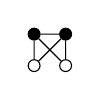
\begin{tikzpicture}[baseline=-1.0mm]
    \newcommand{\sz}{2.0mm}
    \node (r1) at (-\sz, -\sz) [whitedot]{};
    \node (r2) at ( \sz, -\sz) [whitedot]{};
    \node (r3) at ( \sz,  \sz) [blackdot]{};
    \node (r4) at (-\sz,  \sz) [blackdot]{};
    \draw (r1) -- (r4) -- (r3) -- (r2) -- (r4) (r1) -- (r3);
  \end{tikzpicture}
and
  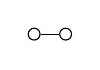
\begin{tikzpicture}[baseline=-1.0mm]
    \newcommand{\sz}{2.0mm}
    \node (r1) at (-\sz, 0) [whitedot]{};
    \node (r2) at ( \sz, 0) [whitedot]{};
    \draw (r1) -- (r2);
  \end{tikzpicture}
respectively.
%
This gives the value $\gamma = 2/3$,
for it balances the contribution of the diagram
  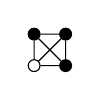
\begin{tikzpicture}[baseline=-1.0mm]
    \newcommand{\sz}{2.0mm}
    \node (r1) at (-\sz, -\sz) [whitedot]{};
    \node (r2) at ( \sz, -\sz) [blackdot]{};
    \node (r3) at ( \sz,  \sz) [blackdot]{};
    \node (r4) at (-\sz,  \sz) [blackdot]{};
    \draw (r1) -- (r2) -- (r3) -- (r4) -- (r1) -- (r3) (r2) -- (r4);
  \end{tikzpicture}
on both sides of \eqref{eq:muexact}.



\subsection{\label{sec:dxi}Expansion of the charging parameter}


We now show how to compute $\partial_\xi B(\vr; 1)$ and $\partial_\xi h(\vr; 1)$,
which are required in the determination of $\gamma$ in \eqref{eq:gamma_muv},
%
Under the charging parameter, \eqref{eq:oz} is modified as
\[
  t(\vr; \xi) = \rho \, c(\vr; \xi) * h(\vr),
\]
So
\begin{equation}
  \partial_\xi t(\vr; 1)
  = \rho \, [\partial_\xi c * (t + c)](\vr, 1).
  \label{eq:ozxi}
\end{equation}

For the closure, we have
\begin{align}
  \partial_\xi c(\vr; 1)
  = [f(\vr) + 1] \, (\partial y/\partial t) \, \partial_\xi t(\vr; 1)
  \notag \\
  + \partial_\xi f(\vr; 1) \, y(\vr) - \partial_\xi t(\vr; 1).
  \label{eq:closurexi}
\end{align}

Once we have solved $c(\vr)$ and $t(\vr)$
from \eqref{eq:oz} and \eqref{eq:closure},
%
we can then solve $\partial_\xi c(\vr; 1)$ and $\partial_\xi t(\vr; 1)$
from \eqref{eq:ozxi} and \eqref{eq:closurexi}, by, e.g., direct iteration.
Then
\begin{align*}
  \partial_\xi B(\vr; 1) &= (\partial B/\partial t) \, \partial_\xi t(\vr; 1), \\
  \partial_\xi h(\vr; 1) &= \partial_\xi c(\vr; 1) + \partial_\xi t(\vr; 1).
\end{align*}



\subsection{\label{sec:genmethod}Generalized method}



Let us now derive \eqref{eq:gamma_muv} from a more general method.
%
We start from differentiating \eqref{eq:muti}:
%
\begin{align}
  -\partial_\xi ( \beta \muex )
  &=
  -\rho \, \int d\vr
    \, \beta \, \partial_\xi u \, g,
    \notag \\
  &=
  \rho \, \int d\vr \,
    \big[
    \partial_\xi c - \partial_\xi B
  - h \, \partial_\xi (t + \partial_\xi B )
    \big],
  \label{eq:dmuti}
\end{align}
%
where we have omitted ``$(\vr; \xi)$'' for convenience.

We now propose a trial expression
%
\begin{align}
  - \beta \mutex
  &=
  \rho \, \int d\vr \,
    \left(
    c
    - \, B
    - \tfrac{1}{2} \, h t
    - \Delta
    \right),
  \label{eq:mutrial}
\end{align}
%
with $\Delta = \Delta(\vr)$ being some correction function.


We wish to choose a $\Delta$ such that \eqref{eq:dmuti} is true:
%
\[
  \partial_\xi \muex =  \partial_\xi \mutex.
\]
%
This yields
\begin{align}
  \int d\vr \, \partial_\xi \Delta
=
  \int d\vr \, h \, \partial_\xi B.
  \label{eq:corr_muv}
\end{align}
%
If we further assume a linear dependence: $\Delta = \gamma_1 \Delta_1$,
then
\begin{align}
  \gamma_1
=
  \frac
  {
    \int \, d\vr \, h \, \partial_\xi B
  }
  {
    \int \, d\vr \, \partial_\xi \Delta_1
  },
  \label{eq:gamma_virial}
\end{align}
%
where we have used $h \, \partial_\xi t = t \, \partial_\xi h = \frac{1}{2} \partial_\xi (t h)$.
%
If $\Delta_1 = h B$, then we recover \eqref{eq:gamma_muv}.
%
Note we can alternatively determine $\gamma$ by the variational principle,
which yields a slightly different formula.
%
We should, however, not consider this possibility below.



\subsection{Compressibility-route chemical potential}

We now extend the above general method to the compressibility route.
%
This requires the derivatives with respect to the density, $\rho$,
instead of $\xi$.
%
We insist that the exact relation
\begin{equation}
  -\partial_\rho (\beta \muex) = \int d\vr \, c(\vr),
  \label{eq:mu_compr}
\end{equation}
is true also for $\mutex$.
%
Then, from \eqref{eq:mutrial}, we get
%
\begin{equation}
  \int \, d\vr \, (1 + \rho \, \partial_\rho) \, \Delta
=
  I_\rho,
  \label{eq:corr_muc}
\end{equation}
%
where
\begin{align*}
I_\rho
&=
\int \, d\vr \,
  \left[
  \frac{1}{2} \, \rho \, (c \, \partial_\rho t - t \, \partial_\rho c)
- \frac{1}{2} \, t \, h
+ \rho \, h \, \partial_\rho B
- B
  \right],
\end{align*}
%
If we assume a linear dependence:
%
$\Delta = \gamma_2 \, \Delta_2$,
then
\begin{equation}
  \gamma_2
=
  \frac
  {
    I_\rho
  }
  {
    \int d\vr \, (1 + \rho \, \partial_\rho) \Delta_2
  },
  \label{eq:gamma_muc}
\end{equation}
where $\Delta_2$ is set to $B$ in non-HNC cases.

Let us now study the integral $I_\rho$.
%
By Fourier transform, we can rewrite it as
\begin{align*}
  I_\rho
&=
  \frac{1}{2} \int \dvk
  \rho^2 \,
  \tilde{h}^2 \,
  \partial_\rho \tilde{c}
  + \int d\vr \,
  (\rho \, h \, \partial_\rho B - B).
\end{align*}
%
The corresponding diagrammatic expansion,
assuming the exact bridge function, $B(\vr)$, is
\begin{align*}
I_\rho
&=
  \int d\vr \,
  \left(
  % diamond
  \frac{1}{2}
  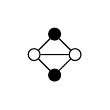
\begin{tikzpicture}[baseline=-1.3mm]
    \newcommand{\sz}{2.6mm}
    \node (r1) at (-\sz,    0) [whitedot]{};
    \node (r2) at ( \sz,    0) [whitedot]{};
    \node (r3) at (   0,  \sz) [blackdot]{};
    \node (r4) at (   0, -\sz) [blackdot]{};
    \draw (r1) -- (r4) -- (r2) -- (r3) -- (r1) -- (r2);
  \end{tikzpicture}
+
  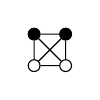
\begin{tikzpicture}[baseline=-1.0mm]
    \newcommand{\sz}{2.0mm}
    \node (r1) at (-\sz, -\sz) [whitedot]{};
    \node (r2) at ( \sz, -\sz) [whitedot]{};
    \node (r3) at ( \sz,  \sz) [blackdot]{};
    \node (r4) at (-\sz,  \sz) [blackdot]{};
    \draw (r1) -- (r4) -- (r3) -- (r2) -- (r4) (r2) -- (r1) -- (r3);
  \end{tikzpicture}
-
\frac{1}{2}
  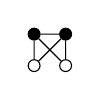
\begin{tikzpicture}[baseline=-1.0mm]
    \newcommand{\sz}{2.0mm}
    \node (r1) at (-\sz, -\sz) [whitedot]{};
    \node (r2) at ( \sz, -\sz) [whitedot]{};
    \node (r3) at ( \sz,  \sz) [blackdot]{};
    \node (r4) at (-\sz,  \sz) [blackdot]{};
    \draw (r1) -- (r4) -- (r3) -- (r2) -- (r4) (r1) -- (r3);
  \end{tikzpicture}
+ \cdots \right)
\notag \\
&= \rho^{-1} \,
  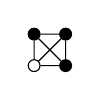
\begin{tikzpicture}[baseline=-1.0mm]
    \newcommand{\sz}{2.0mm}
    \node (r1) at (-\sz, -\sz) [whitedot]{};
    \node (r2) at ( \sz, -\sz) [blackdot]{};
    \node (r3) at ( \sz,  \sz) [blackdot]{};
    \node (r4) at (-\sz,  \sz) [blackdot]{};
    \draw (r1) -- (r4) -- (r3) -- (r2) -- (r4) (r2) -- (r1) -- (r3);
  \end{tikzpicture} + \cdots,
  %\label{eq:Iqhnc}
\end{align*}
%
where the diagrams are implicitly labeled, and hence
have no additional symmetry numbers.
%
Thus, to cancel this term in the low density limit,
we can set $\Delta_2 = h\, B$, with $\gamma_2 = 2/3$,
as given by \eqref{eq:gamma_muc}.
%
In practice, for the hard-sphere fluid,
we find it to be more effective to set
$\Delta_2 = B$, when $B$ does not vanish.



In the HNC case, $B(\vr) = 0$, and
\[
I_\rho
=
  \frac{1}{2} \, \rho^{-1} \,
  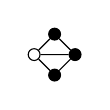
\begin{tikzpicture}[baseline=-1.3mm]
    \newcommand{\sz}{2.6mm}
    \node (r1) at (-\sz,    0) [whitedot]{};
    \node (r2) at ( \sz,    0) [blackdot]{};
    \node (r3) at (   0,  \sz) [blackdot]{};
    \node (r4) at (   0, -\sz) [blackdot]{};
    \draw (r1) -- (r4) -- (r2) -- (r3) -- (r1) -- (r2);
  \end{tikzpicture}
  + \cdots,
\]
which does not vanish.
%
This means that the classic formula \eqref{eq:muhnc}
is applicable only to the virial route
but not to the compressibility route.
%
To make a correction, we set
\begin{equation}
  \Delta_2^{\mathrm{HNC}} = c - (1 + \rho f*f) f,
  \label{eq:Delta2_hnc}
\end{equation}
in place of $B$.

A natural extension is to design a $\Delta$ that simultaneously satisfies
both \eqref{eq:corr_muv} and \eqref{eq:corr_muc}.
%
That is, we set
\begin{equation}
  \Delta = \gamma_1 \, \Delta_1 + \gamma_2 \, \Delta_2,
  \label{eq:mucv_consistent}
\end{equation}
and then solve $\gamma_1$ and $\gamma_2$.
%
In practice,
the chemical potential resulting from this equation
is rather similar to that from \eqref{eq:corr_muc},
in the case of three-dimensional hard-sphere fluid.



Another possibility is to use a trial functional form
different from \eqref{eq:mutrial}.
%
Using the compressibility-route for example,
we can consider a linear interpolation
of $f$,
$\rho \, (f*f) f =
  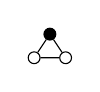
\begin{tikzpicture}[baseline=-1.4mm]
    \newcommand{\sz}{2.0mm}
    \node (r1) at (-\sz, -\sz) [whitedot]{};
    \node (r2) at ( \sz, -\sz) [whitedot]{};
    \node (r3) at (   0, 0.5*\sz) [blackdot]{};
    \draw (r1) -- (r2) -- (r3) -- (r1);
  \end{tikzpicture}$,
$c$, and $\rho \, \partial_\rho \, c$:
\begin{align}
  -\beta \, \mutex
=
  \int \, d\vr \,
  \left\{
  \frac{\rho}{2} \, (f + c)
+ \frac{\rho^2}{12} \, \Big[(f*f) \, f - \partial_\rho c\Big]
  \right\},
  \label{eq:muc_series}
\end{align}
which satisfies the boundary conditions:
\begin{equation}
  \begin{split}
  - \partial_{\rho}( \beta \, \mutex )
  \hphantom{ \Big|_{\rho = 0} }
&=
  \int d\vr \, c,
%
  \\
  - \partial_{\rho \rho}( \beta \, \mutex )
  \hphantom{ \Big|_{\rho = 0} }
&=
  \int d\vr \, \partial_\rho c,
  \\
%
    - \partial_\rho( \beta \, \mutex )
  \Big|_{\rho = 0}
&=
  \int d\vr \, f,
%
  \\
  - \partial_{\rho \rho}( \beta \, \mutex )
  \Big|_{\rho = 0}
&=
  \int d\vr \, f \, (f * f).
  \end{split}
  \label{eq:muc_boundary}
\end{equation}


% Alternatively, we can use a rational approximation
% \begin{align}
%   -\beta \, \mutex
% =
%   \frac{ A_1 \rho + A_2 \rho^2 + A_3 \rho^3 }
%   {1 + B_1 \rho },
%   \label{eq:mut_rational}
% \end{align}
% and solve the coefficients $A_1$, $A_2$, $A_3$, and $B_1$
% from \eqref{eq:muc_boundary}.
% %\begin{align}
% %  -\beta \, \mutex
% %=
% %  \int \, d\vr \,
% %  \left[
% %    \rho \, f
% %+ \frac{\rho^2}{2} \, (f*f) \, f
% %  \right]
% %+ \frac{ \rho \, C_2^2 }
% %  { C_2 + \rho \, \partial_\rho C_2 },
% %  \label{eq:muc_power}
% %\end{align}
% %with
% %\begin{equation}
% %  C_2 \equiv \int d\vr \, \big[ c - (1 + \rho f * f) f\big].
% %  \label{eq:C2pdef}
% %\end{equation}



\subsection{\label{sec:c-pres}Compressibility-route pressure}

The above techniques can be used to
compute the compressibility-route pressure.
%
We now construct a trial function
\begin{align}
  \beta \, \Pex
&=
 -\frac{ \rho^2 }{ 2 }
 \int d\vr \, (c - h c - \Delta)
 \notag \\
& \quad + \int \dvk \,
  \big[
    \log( 1 - \rho \tilde{c} )
    + \rho \tilde{c}
  \big].
  \label{eq:Ptrial}
\end{align}
%
The case of $\Delta = 0$ recovers the exact formula
for the PY closure\cite{baxterpressure}.

Differentiating with respect to $\rho$ yields
%
\begin{align}
  \partial_\rho ( \beta \, \Pex )
&=
 -\rho \int d\vr \, c
 \notag \\
&\hphantom{=}
 - J_\rho
 + \int d\vr \,
  \left(
    \rho + \frac{ \rho^2 }{ 2 }  \, \partial_\rho
  \right) \, \Delta,
  \label{eq:dPtrial}
\end{align}
%
where
\begin{align*}
  J_\rho
  &= \frac{\rho^2}{2}
  \big(
 \partial_\rho c
 - c \partial_\rho t
 + t \partial_\rho c
\big)
\notag \\
&= \frac{\rho^2}{2}
 \Big\{
 (1+ f)
 \big[
  (1+t) \partial_\rho w
  -w\partial_\rho t
  \big]
 \Big\},
\end{align*}
and $w = y - 1 - t$.
%
Thus, to ensure the exact relation
\[
\partial_\rho (\beta \Pex)
= -\rho \int d\vr \, c,
\]
we set
\[
  \int d\vr \,
  \left(\rho + \frac{\rho^2}{2} \partial_\rho\right) \Delta
  = J_\rho.
\]
With
$\Delta = \theta \, \Delta_3$,
we get
\begin{equation}
  \theta
=
  \frac
  {
    J_\rho
  }
  {
    \int d\vr \,
    \left( \rho + \frac{\rho^2}{2} \, \partial_\rho \right)
    \Delta_3
  }.
  \label{eq:theta}
\end{equation}
%
Particularly, we choose $\Delta_3 = (1+ f) (1 + t) w$.

Similar to the case of chemical potential,
we have an interpolation formula
\begin{equation}
\beta \Pex = -\int d\vr \,
\left[
  \frac{3 \rho^2}{20} f
+ \frac{7 \rho^2}{20} c
+ \frac{\rho^3}{30} f (f * f)
- \frac{\rho^3}{20} \partial_\rho c
\right].
\label{eq:P_series}
\end{equation}
%
which satisfies the boundary conditions
% Alternatively, we can set
% \begin{equation}
%   \beta \Ptex
% =
% \frac{ A_2 \rho^2 + A_3 \rho^3 + A_4 \rho^4 }
% { 1 + B_1 \rho },
% \label{eq:Pt_rational}
% \end{equation}
% and solve $A_2$, $A_3$, $A_4$, and $B_1$ from
% the boundary conditions
%
\begin{equation}
  \begin{split}
  - \partial_{\rho}( \beta \, \Ptex )
  \hphantom{ \Big|_{\rho = 0} }
&=
  \rho \, \int d\vr \, c,
  \\
%
  - \partial_{\rho \rho}( \beta \, \Ptex )
  \hphantom{ \Big|_{\rho = 0} }
&=
  \int d\vr \,
    (1 + \rho \, \partial_\rho) \, c,
  \\
%
  - \partial_\rho( \beta \, \Ptex )
  \Big|_{\rho = 0}
&=
  \rho \, \int d\vr \, f,
  \\
%
  - \partial_{\rho \rho}( \beta \, \Ptex )
  \Big|_{\rho = 0}
&=
  \int d\vr \,
  [1 + 2 \, \rho \, (f*f) ] \, f.
  \end{split}
  \label{eq:Pc_boundary}
\end{equation}






\subsection{Virial series}


We computed the reference values from the virial series.
%
We write pressure as
\[
  \beta P = \sum_{n = 1}^{\infty} B_n \, \rho^n.
\]
%
Using $\partial_\rho P = \rho \, \partial_\rho \mu$,
we get an expression of chemical potential
\begin{equation}
  \beta \muex = - \sum_{n = 2}^\infty \frac{n B_n}{n - 1} \rho^{n - 1}.
  \label{eq:muvirialseries}
\end{equation}
%
In the HNC case for the three-dimensional hard-sphere fluid,
the virial diverges at high orders.
%
Thus, we used the truncated series at two orders
and then take the average.
%
For the compressibility route,
we used the average of the 7th and 9th order results.
%
For the virial route,
we used the average of the 12th and 13th order results.



\subsection{\label{sec:sc} Self-consistent integral equation}



One application of computing chemical potential and pressure
is to provide criteria that can be used
to adjust parameters in self-consistent integral equations.
%
Without the exact bridge function, integral equations
are inevitably approximate, and thus contains some self-inconsistency.
%
By enforcing the self-consistency
of some thermodynamic quantity,
we can usually improve the accuracy of integral equations.

For the pressure, we have
\begin{equation}
  \partial_\rho \big[ \beta P^{(c)} \big] = 1 - \rho \int c(\vr) \, d\vr,
  \label{eq:dPcomp}
\end{equation}
for the compressibility route, with $D$ being the dimension, and
%
\begin{equation}
  \beta P^{(v)} = \rho + \frac{\rho^2}{2D} \int \vr \cdot \nabla f(\vr) y(\vr) \, d\vr,
  \label{eq:Pvirial}
\end{equation}
for the virial route.
%
A more convenient form for direct comparison with \eqref{eq:dPcomp} is
\begin{equation}
  \partial_\rho \big[ \beta P^{(v)} \big] =
    \frac{ 2\beta P^{(v)} }{ \rho } - 1
    + \frac{\rho^2}{2D} \int \vr \cdot \nabla f(\vr) \, \partial_\rho y(\vr) \, d\vr,
  \label{eq:dPvirial}
\end{equation}
where $\partial_\rho y(\vr)$ can be computed using a technique similar to that in Sec. \ref{sec:dxi}.
%
In a self-consistent integral equation,
we choose parameters such that
$\partial_\rho P^{(c)}$
is equal to
$\partial_\rho P^{(v)}$.


Since we are interested in the chemical potential here,
it would be better if we compare $\mu$, instead of $P$, from the two routes.
%
Using \eqref{eq:dPcomp} and $\partial_\rho P = \rho \, \partial_\rho \mu$,
we have, for the compressibility route,
\begin{equation}
  -\partial_\rho \big[ \beta \mu^{(c)} \big]
  =  -\rho^{-1} + \int c(\vr) \, d\vr.
  \notag
\end{equation}
For the virial route, we have
\begin{equation}
  -\partial_\xi \big[ \beta \mu^{(v)} \big]
  =  \rho \int \partial_\xi f(\vr; 1) \, y(\vr) \, d\vr.
  \notag
  \label{eq:dmudxi}
\end{equation}

Again, for better comparison,
we insist the agreement of
\begin{equation}
  -\partial^2_{\rho \, \xi} \big[ \beta \mu^{(c)} \big]
  = \int \partial_\xi c(\vr; 1) \, d\vr,
  \label{eq:ddmuc}
\end{equation}
and
\begin{equation}
  -\partial^2_{\xi \, \rho} \big[ \beta \mu^{(v)} \big]
  =  \int
  \partial_\xi f(\vr; 1) \,
  (1 + \rho \, \partial_\rho) \, y(\vr)
  \, d\vr.
  \label{eq:ddmuv}
\end{equation}
%

In Appendix \ref{apd:sc},
  we describe a practical procedure
  to adjust parameters in integral equations
  to enforce the above consistency conditions.





\section{Results}



\subsection{Chemical potential}

We computed the chemical potential from a few integral equations.
%
%the PY ($y = 1 + t$), quadratic ($y = 1 + t + \eta t^2/2$),
%Rowlinson [$y = 1 + t + \eta (\exp t - 1 - t)$],
%and
%Hutchinson-Conkie [HC, $y = (1+s t)^{1/s}$]
%integral equations.
%The parameters in the latter equations, $\eta$ and $s$,
%were determined self-consistently using the method in Sec. \ref{sec:sc}.
%
To evaluate the accuracy,
we prepared the following two reference values.
%
The first reference is the chemical potential computed from
the first twelve known virial coefficients
using \eqref{eq:muvirialseries}.
%
The second reference concerns the consistency
regarding a variation of the charging parameter, $\xi$:
%
we compute the chemical potential $\supex{\mu'}$
under $\xi' = 1 - \delta \xi$
and then see if $(\muex - \supex{\mu'})/\delta \xi$
matches
$\partial_\xi \muex$ given by \eqref{eq:dmuti}.
%
Note, in the $\xi' \ne 1$ case, we simply borrow the $\gamma$ value
from the $\xi = 1$ case without using
\eqref{eq:gamma_muv} or \eqref{eq:gamma_muc}
(which is an assumption of the derivation).


\subsubsection{HNC closure}


As shown in Fig. \ref{fig:muhnc},
for the HNC closure,
%
the results from the classic formula \eqref{eq:muhnc}
coincide with the virial-route results,
%
while the results of \eqref{eq:gamma_muc} and \eqref{eq:muc_series}
agree well with the compressibility-route result.
%


\begin{figure}[h]
  \makebox[\linewidth][c]{
    \includegraphics[angle=0, width=0.9\linewidth]{fig/muhnc.pdf}
  }
  \caption{
    \label{fig:muhnc}
    Chemical potential from the HNC closure.
    %(a) $\muex$. (b) $d\muex/d\xi$.
    %In (a), the compressibility and virial results
    %for the HNC closures
    %(dashed and dotted lines, respectively)
    %were computed from the first 64th virial coefficients.
    %The result of Mayer sampling (solid line)
    %was computed from the first 12th virial coefficients.
  }
\end{figure}




\subsubsection{PY closure}

\begin{figure}[h]
  \makebox[\linewidth][c]{
    \includegraphics[angle=0, width=0.9\linewidth]{fig/mupy.pdf}
  }
  \caption{
    \label{fig:mupy}
    Chemical potential from the PY closure.
    (a) $\muex$. (b) $d\muex/d\xi$.
    %In (a), the compressibility and virial results
    %for the PY closures
    %(dashed and dotted lines, respectively)
    %were computed from the first 64th virial coefficients.
    %That of Mayer sampling (Reference, solid line)
    %was computed from the first 12th virial coefficients.
  }
\end{figure}



The results of the PY closure are shown in Fig. \ref{fig:mupy}.
%
If the approximation \eqref{eq:approxhB} is used,
a nonzero $\gamma$ is necessary
to produce a reasonable chemical potential at a high density.
%
The value $\gamma = 2/3$ gives good results.
%
For comparison,
the results of \eqref{eq:gamma_muv}
appear to be inferior,
whereas those of \eqref{eq:gamma_muc} are better.
%
This is due to the internal inconsistency
as discussed below.
%
Besides,
Eq. \eqref{eq:muc_series}, which is derived for the compressibility-route,
and
Eq. \eqref{eq:mucv_consistent}, which is consistent for both
the compressibility and virial routes,
give good results.
%
This shows that the compressibility-route-based formulae
are useful in improving the accuracy of chemical potential.



The apparently inferior chemical potential from \eqref{eq:gamma_muv}
is a result of the internal inconsistency of the integral equation.
%
As shown in Fig. \ref{fig:mupy}(b),
for $d\muex/d\xi$,
only the results from \eqref{eq:gamma_muv} and \eqref{eq:mucv_consistent},
which are virial-route consistent,
agree well with the reference values
computed from \eqref{eq:dmuti}.
%



%The $\gamma$ values
%%%
%%\eqref{eq:gamma_muv} achieves better agreement
%%between $\muex(1) - \muex(1 - \delta \xi)$ and $(d\muex/d\xi) \, \delta \xi$
%
%\begin{figure}[h]
%  \makebox[\linewidth][c]{
%    \includegraphics[angle=0, width=1.0\linewidth]{fig/mugamma.pdf}
%  }
%  \caption{
%    \label{fig:mugamma}
%    The value $\gamma$ as a function of the density, $\rho$,
%    in a few closures.
%  }
%\end{figure}
%
% The value $\gamma$ computed from \eqref{eq:gamma_muv}
% starts with $2/3$ in the low-density region,
% %
% and then decreases slightly with the density, $\rho$,
% as shown in Fig. \ref{fig:mugamma}.
% %



\subsubsection{Self-consistent closures}


\begin{figure}[h]
  \makebox[\linewidth][c]{
    \includegraphics[angle=0, width=0.9\linewidth]{fig/musqr.pdf}
  }
  \caption{
    \label{fig:musqr}
    Chemical potential $\muex$ from the self-consistent quadratic closure.
    (a) $\partial_\rho P$-consistent, Eqs. \eqref{eq:dPcomp} and \eqref{eq:dPvirial}.
    (b) $\partial_{\rho \xi} \mu$-consistent, Eqs. \eqref{eq:ddmuc} and \eqref{eq:ddmuv}.
  }
\end{figure}


We tested the formulae on a few self-consistent closures,
which are intended to improve the accuracy of the PY and HNC closures.
%
Below we used the self-consistent quadratic closure ($y = 1 + t + \eta \, t^2$) as an example.
%
The parameter $\eta$ is determined self-consistently using the method in Sec. \ref{sec:sc}
and Appendix \ref{apd:sc}.
%
As shown in Fig. \ref{fig:musqr},
%
in the $\partial_\rho P$-consistent version,
the compressibility-route based formulae,
\eqref{eq:gamma_muc} and \eqref{eq:muc_series},
are more accurate than the virial-route base one,
\eqref{eq:gamma_muv}.
%
However, the opposite is true in the $\partial_{\rho \xi} \mu$-consistent version.
%
%Further, we find that if the parameters in the integral equations
%are adjusted based on the consistency of $\partial^2_{\rho \, \xi} \mu$
%[using \eqref{eq:ddmuc} and \eqref{eq:ddmuv}]
%instead of that of $\partial_\rho P$
%[using \eqref{eq:dPcomp} and \eqref{eq:dPvirial}],
%the chemical potential from \eqref{eq:approxhB} and \eqref{eq:gamma_muv} are improved.
%



\subsubsection{Explicit bridge function}


We computed the chemical potential from the closure with
the explicit bridge function, $B(\vr)$,
which was obtained from Mayer sampling
of the density components as $B(\vr) = \sum_{l = 2}^{6} B_l(\vr) \rho^l$.
%
Since $\partial_\xi B(\vr; 1)$ was unavailable in this case,
we used the predefined values $\gamma = 2/3-0.09\rho$
instead of \eqref{eq:gamma_muv}.
%
However, $\partial_\rho B(\vr) = \sum_{l = 2}^{6} l \, B_l(\vr) \rho^{l-1}$
was available,
and \eqref{eq:gamma_muc} and \eqref{eq:muc_series} were applicable.
%
and the results are shown in Fig. \ref{fig:muBr}.
%
Clearly, $\gamma = 2/3$ yields better results than $\gamma = 0$,
whereas the results from $\gamma = 2/3-0.09\rho$
are even better and almost indistinguishable from the reference.
%
The results from \eqref{eq:gamma_muc} and \eqref{eq:muc_series}
show only small deviation at large density.
%
\begin{figure}[h]
  \makebox[\linewidth][c]{
    \includegraphics[angle=0, width=1.0\linewidth]{fig/muBr.pdf}
  }
  \caption{
    \label{fig:muBr}
    Chemical potential from the closure with the explicit bridge function $B(\vr)$.
  }
\end{figure}




\subsection{Pressure}


The compressibility-route pressure is computed from the methods in Sec. \ref{sec:c-pres}.
%
As shown in Fig. \ref{fig:Phnc}, for the HNC closure,
%
both \eqref{eq:Ptrial}
[with $\theta = 1/2$, or determined from \eqref{eq:theta}],
and \eqref{eq:P_series},
give good results for the pressure.
%


\begin{figure}[h]
  \makebox[\linewidth][c]{
    \includegraphics[angle=0, width=1.0\linewidth]{fig/Phnc.pdf}
  }
  \caption{
    \label{fig:Phnc}
    Compressibility-route pressure from the HNC closure.
  }
\end{figure}






\section{Discussions}

In summary, we have presented a simple method
of computing the chemical potential and pressure
from an arbitrary integral equation.
%
The method, however, requires one to solve
an additional integral equation
regarding derivatives with respect to $\xi$ or $\rho$.
%
%We can, however, circumvent the problem by choosing
%an empirical $\gamma$, as we did in the last example [\ref{fig:muBr}].
%%
If this is inconvenient,
the values $\gamma \approx 2/3$ for chemical potential
or $\theta \approx 1/2$ for pressure
seem to work well for the hard-sphere fluid.
%%
However, these empirical values might not be
applicable to more complex fluids.



\appendix

\section{\label{apd:sc}
Parameter determination of self-consistent integral equations}

To achieve the consistency of \eqref{eq:dPcomp} and \eqref{eq:dPvirial}
in an integral equation with an adjustable parameter $\eta$,
we update $\eta$ as $\eta \rightarrow \eta + \Delta \eta$,
with $\Delta \eta$ computed from equating the following two equations
%
\begin{align*}
  \partial_\rho \big[ \beta P^{(c)} \big]
&\approx
  1 - \rho \int d\vr \, c
  - \Delta \eta \, \rho
  \int d\vr \, (f + 1) \, (dy/dt) \, \partial_\rho t,
\\
  \partial_\rho \big[ \beta P^{(v)} \big]
&\approx
  1 + (\rho/D) \int d\vr \, \vr \cdot \nabla f \,
  \big[ y + (\rho/2) \, (dy/dt) \, \partial_\rho t \big]
  \\
&  + \Delta \eta
  \, (\rho/D) \int d\vr \, \vr \cdot \nabla f \,
  \big[ \partial_\eta y + (\rho/2) \, \partial_\eta (dy/dt) \, \partial_\rho t \big].
\end{align*}

Similarly, for \eqref{eq:ddmuc} and \eqref{eq:ddmuv},
we have
\begin{align*}
  -\partial^2_{\rho \, \xi} \big[ \beta \mu^{(c)} \big]
  &= \int d\vr \, \partial_\xi c \, d\vr \\
  & + \Delta \eta \, \int d\vr \big[
      (\partial_\xi f) \, y + (1 + f) \, (dy/dt) \, \partial_\xi t
    \big],
\\
  -\partial^2_{\xi \, \rho} \big[ \beta \mu^{(v)} \big]
  &=  \int d\vr \,
  \partial_\xi f \,
  \big[ y + \rho \, (dy/dt) \, \partial_\rho t \big]
  \\
& + \Delta \eta \, \int d\vr \,
  \partial_\xi f \,
  \big[ \partial_\eta y + \rho \, \partial_\eta (dy/dt) \, \partial_\rho t \big],
\end{align*}
and $\Delta \eta$ is solved from equating the two.


\bibliography{liquid}
\end{document}

